\chapter{Problem 2}
\section{Problem statement}

Team needs to form a use-case model \cite{use-case-diagram} for METRICSTICS where use-case scenarios are specified along with their description having actors involved in those use-cases.

\section{Use Case Model} 
    \begin{figure}[H]
        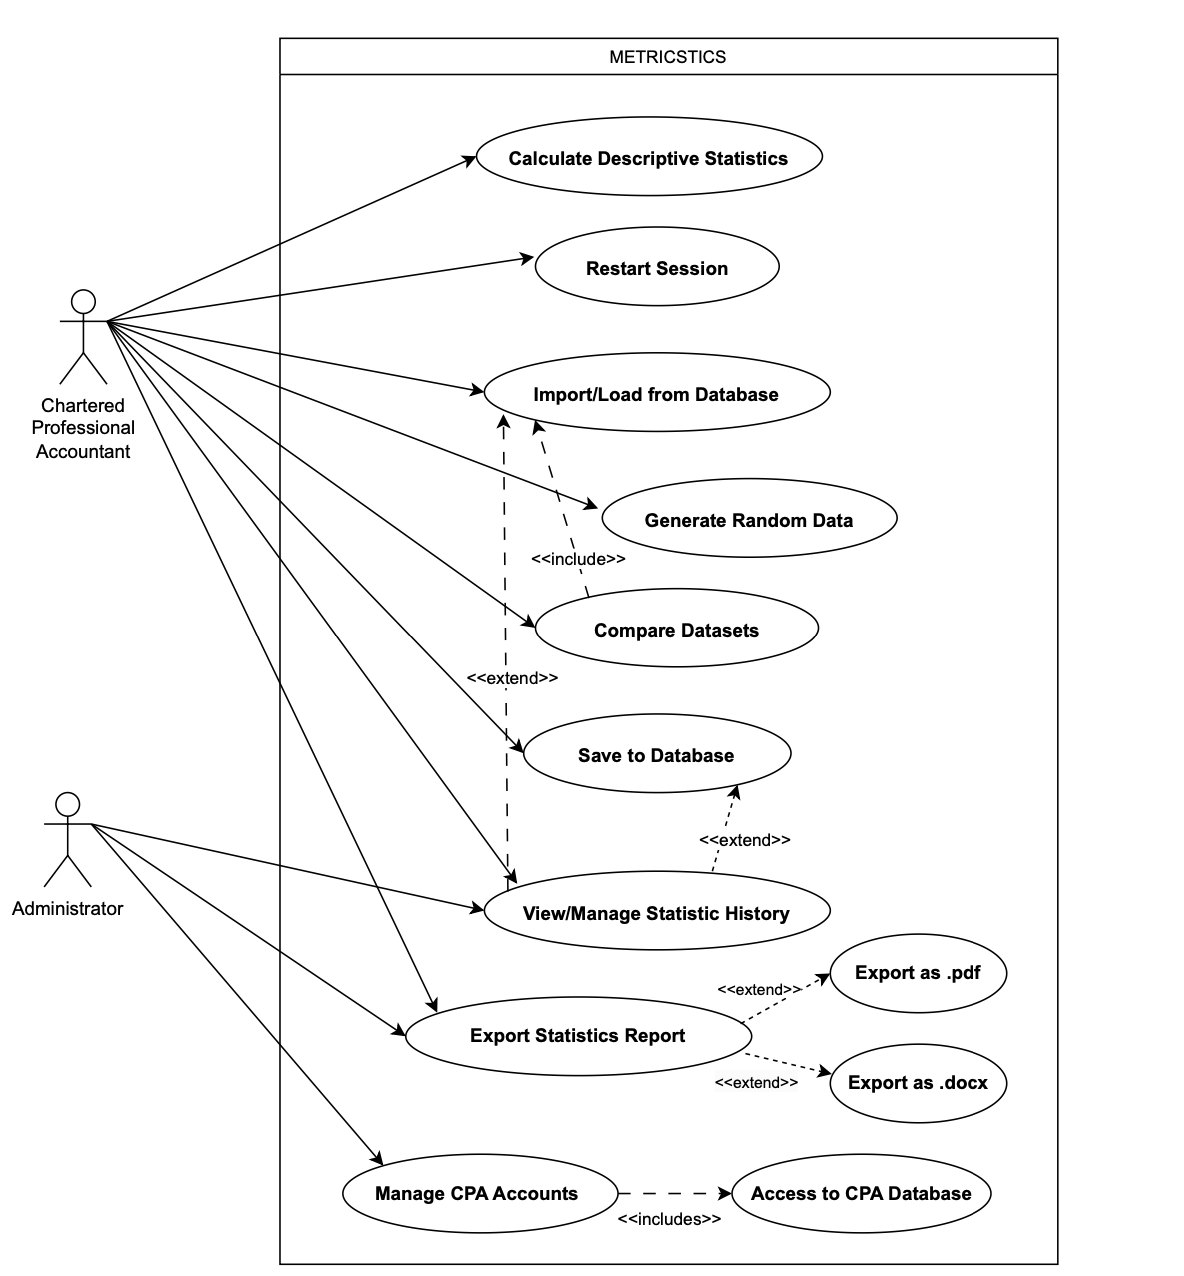
\includegraphics[width=13.3cm]{images/use_case_model.png}
        \caption{Use Case Model}
    \end{figure}

\section{Description Tables}

\begin{table}[H]
\centering
\def\arraystretch{1.5}
\begin{tabular}{|l|p{4.4in}|}
\hline
\ac{UC} ID & UC-1\\ \hline
Use Case Name & Calculate Descriptive Statistics\\ \hline
Primary Actors & CPA\\ \hline
Priority & High\\ \hline
Description & The CPA enters a collection of data values into METRICSTICS, and the system computes and displays the data's values for minimum, maximum, mode, median, mean, mean absolute deviation, and standard deviation.\\ \hline
Pre-conditions & The CPA is logged into the METRICSTICS system.\\ \hline
Post-conditions & The descriptive statistics for the entered data are displayed to the CPA.\\ \hline
Normal Flow & 1. \ac{CPA} logs into METRICSTICS.
     \newline 2. CPA selects the $"Calculate Descriptive Statistics"$ option.
     \newline 3. CPA enters the data values.
     \newline 4. The system computes and displays the descriptive statistics.
    \\ \hline
\end{tabular}
\caption{Use Case-1, Calculate Descriptive Statistics}
\end{table}

\begin{table}[H]
\centering
\def\arraystretch{1.5}
\begin{tabular}{|l|p{4.5in}|}
\hline
Use Case ID & UC-2\\ \hline
Use Case Name & Save to Database\\ \hline
Primary Actors & CPA\\ \hline
Priority & Medium\\ \hline
Description & The CPA saves a collection of data values along with the descriptive \mbox{statistics} that go along with it to a file for later use or study.\\ \hline
Pre-conditions & The CPA has calculated descriptive statistics for a set of data\\ \hline
Post-conditions & Data and associated statistics are saved to the database.\\ \hline
Normal Flow & 1. CPA calculates descriptive statistics.
     \newline 2. CPA selects the $"Save To Database"$ option.
     \newline 3. CPA provides a name and description for the saved dataset.
     \newline 4. System saves the data and statistics to the database.
    \\ \hline
\end{tabular}
\caption{Use Case-2, Save to Database}
\end{table}

\begin{table}[H]
\centering
\def\arraystretch{1.5}
\begin{tabular}{|l|p{4.5in}|}
\hline
Use Case ID & UC-3\\ \hline
Use Case Name & Import/Load From Database\\ \hline
Primary Actors & CPA\\ \hline
Priority & High\\ \hline
Description & The CPA loads into METRICSTICS for further analysis a previously saved set of data values and the related descriptive statistics.\\ \hline
Pre-conditions & The CPA is logged into the METRICSTICS system.\\ \hline
Post-conditions & The selected dataset and its associated statistics are loaded for analysis.\\ \hline
Normal Flow & 1. CPA logs into METRICSTICS.
     \newline 2. CPA selects the $"Import/Load From Database"$ option.
     \newline 3. CPA selects a previously saved dataset.
     \newline 4. The system loads the data and associated statistics.
    \\ \hline
\end{tabular}
\caption{Use Case-3, Import/Load From Database}
\end{table}

\begin{table}[H]
\centering
\def\arraystretch{1.5}
\begin{tabular}{|l|p{4.5in}|}
\hline
Use Case ID & UC-4\\ \hline
Use Case Name & Restart Session\\ \hline
Primary Actors & CPA\\ \hline
Priority & Low\\ \hline
Description & The CPA can restart the whole calculation session from the start without saving any unnecessary data from the current session.\\ \hline
Pre-conditions & The CPA is in an active calculation session.\\ \hline
Post-conditions & The current session is reset, and no data is saved.\\ \hline
Normal Flow & 1. CPA selects the $"Restart Session"$ option.
     \newline 2. The system clears the current session and resets it.
    \\ \hline
\end{tabular}
\caption{Use Case-4, Restart Session}
\end{table}


\begin{table}[H]
\centering
\def\arraystretch{1.5}
\begin{tabular}{|l|p{4.5in}|}
\hline
Use Case ID & UC-5\\ \hline
Use Case Name & Generate Random Data\\ \hline
Primary Actors & CPA\\ \hline
Priority & Medium\\ \hline
Description & The CPA specifies the range and number of data values, and \mbox{METRICSTICS} creates a set of random data values that may be tested or used in demonstrations.\\ \hline
Pre-conditions & The CPA is logged into METRICSTICS.\\ \hline
Post-conditions & A set of random data values is generated based on CPA's specifications.\\ \hline
Normal Flow & 1. CPA logs into METRICSTICS.
     \newline 2. CPA selects the $"Generate Random Data"$ option.
     \newline 3. CPA specifies the range and number of data values.
     \newline 4. The system generates random data based on the CPA's specifications.
    \\ \hline
\end{tabular}
\caption{Use Case-5, Generate Random Data}
\end{table}


\begin{table}[H]
\centering
\def\arraystretch{1.5}
\begin{tabular}{|l|p{4.5in}|}
\hline
Use Case ID & UC-6\\ \hline
Use Case Name & Compare Datasets\\ \hline
Primary Actors & CPA\\ \hline
Priority & Medium\\ \hline
Description & The system compares the descriptive statistics of two or more sets of data values to find similarities and differences.\\ \hline
Pre-conditions & The CPA has loaded multiple datasets for comparison.\\ \hline
Post-conditions & Comparison results are displayed to the CPA.\\ \hline
Normal Flow & 1. CPA loads multiple datasets for comparison.
     \newline 2. CPA selects the $"Compare Datasets"$ option.
     \newline 3. System analyzes and displays the comparisons.
    \\ \hline
\end{tabular}
\caption{Use Case-6, Compare Datasets}
\end{table}


\begin{table}[H]
\centering
\def\arraystretch{1.5}
\begin{tabular}{|l|p{4.5in}|}
\hline
Use Case ID & UC-7\\ \hline
Use Case Name & View/Manage Statistic History\\ \hline
Primary Actors & CPA, Administrator\\ \hline
Priority & Medium\\ \hline
Description & The CPA and the administrator can view/manage the descriptive statistics on data sets.\\ \hline
Pre-conditions & The CPA or administrator is logged into METRICSTICS.\\ \hline
Post-conditions & Descriptive statistics history is viewed or managed as required.\\ \hline
Normal Flow & 1. CPA or administrator logs into METRICSTICS.
     \newline 2. CPA or administrator selects the $"View/Manage Statistic History"$ \mbox{option}.
     \newline 3. The system displays the history or allows management actions.
    \\ \hline
\end{tabular}
\caption{Use Case-7, View/Manage Statistic History}
\end{table}


\begin{table}[H]
\centering
\def\arraystretch{1.5}
\begin{tabular}{|l|p{4.5in}|}
\hline
Use Case ID & UC-8\\ \hline
Use Case Name & Export Statistics Report\\ \hline
Primary Actors & CPA, Administrator\\ \hline
Priority & Medium\\ \hline
Description & The CPA and the administrator can export a given statistical report to an external data destination connected to the METRICSTICS system.\\ \hline
Pre-conditions & A statistical report is available for export.\\ \hline
Post-conditions & The statistical report is exported to an external destination.\\ \hline
Normal Flow & 1. CPA or administrator selects the $"Export Statistics Report"$ option.
     \newline 2. CPA or administrator chooses the format for export (e.g., PDF, DOCX).
     \newline 3. The system exports the report to the selected format.
    \\ \hline
\end{tabular}
\caption{Use Case-8, Export Statistics Report}
\end{table}


\begin{table}[H]
\centering
\def\arraystretch{1.5}
\begin{tabular}{|l|p{4.5in}|}
\hline
Use Case ID & UC-9\\ \hline
Use Case Name & Manage CPA Accounts\\ \hline
Primary Actors & Administrator\\ \hline
Priority & High\\ \hline
Description & The Administrator has access to manage the CPA accounts set up on the system.\\ \hline
Pre-conditions & The Administrator is logged into METRICSTICS.\\ \hline
Post-conditions & CPA accounts are managed as required.\\ \hline
Normal Flow & 1. Administrator logs into METRICSTICS.
     \newline 2. The administrator selects the $"Manage CPA Accounts" option$.
     \newline 3. The system provides options for managing CPA accounts.
    \\ \hline
\end{tabular}
\caption{Use Case-9, Manage CPA Accounts}
\end{table}


\begin{table}[H]
\centering
\def\arraystretch{1.5}
\begin{tabular}{|l|p{4.5in}|}
\hline
Use Case ID & UC-10\\ \hline
Use Case Name & Access To CPA Database\\ \hline
Primary Actors & Administrator\\ \hline
Priority & High\\ \hline
Description & This use case simply gives the Administrator access to the CPA database connected with the METRICSTICS system to store details of its CPAs.\\ \hline
Pre-conditions & The Administrator is logged into METRICSTICS.\\ \hline
Post-conditions & The Administrator has access to the CPA database.\\ \hline
Normal Flow & 1. Administrator logs into METRICSTICS.
     \newline 2. The administrator selects the $"Access To CPA Database"$ option.
     \newline 3. The system grants access to the CPA database for management purposes.
    \\ \hline
\end{tabular}
\caption{Use Case-10, Access To CPA Database}
\end{table}